\documentclass[thesis.tex]{subfiles}
\def\x{\mathbf{x}}
\def\p{\mathbf{p}}
\def\c{\mathbf{c}}
\def\sigmacellj{\boldsymbol{\sigma}_{\text{cell},j}}
\def\sigmacenter{\boldsymbol{\sigma}_\text{center}}
\begin{document}
\chapter{Proposed descriptor}
%
Our proposed descriptor consists of weighted smooth histograms computed for several \textit{cells} arranged in a grid. We define the $j$'th cell histogram $H_j$ as
%
\begin{align}
\label{eq:proposed_histogram}
H_j(f_i) = \int F(\x) A_j (\x) P (\x) B(\x; f_i,f) \,\text{d} \x
\end{align}
%
where
%
\begin{itemize}
\item[] $f_i$ is a bin center,
\item[] $f$ is a value function defining the bin domain,
\item[] $F$ is a magnitude function,
\item[] $A_j$ is a cell aperture function,
\item[] $P$ is a center aperture function, and
\item[] $B$ is a binning aperture function.
\end{itemize}
%
Note that this definition is similar to the galaxy descriptor \cite{pedersen2013shape}, except we consider several histograms with their own aperture functions $A_j$ and add the additional center aperture function $P$. The descriptor $D$ is constructed by concatenating all $n$ bin values of all $m$ cell histograms:
%
\begin{align}
\label{eq:proposed_descriptor}
D = \Bigl( \left(H_1(f_1) \cdots H_1(f_n)\right) \cdots (H_m(f_1) \cdots H_m(f_n)) \Bigr)
\end{align}
%
The five functions above can be seen as the components that make up our descriptor, and we consider different choices for each. The functions depend on numerous additional parameters, which we define and describe further in this chapter. These parameters will be subject to a parameter study for each of our applications in order to get the most optimal descriptor for the specific application. The parameter studies are described in \Cref{sec:icParameterStudy,sec:odParameterStudy}.
%
\section{Value and magnitude functions}
\label{sec:valueMagnitudeFunctions}
%
The choice of value and magnitude functions are closely connected, as we wish the magnitude function to weight the histogram values according to their importance for the local image structure. The by far most common choice in literature \cite{lowe2004distinctive,ke2004pca,mikolajczyk2005performance,tola2008fast} is using gradient orientation $\Theta$ as value function and gradient magnitude $M$ as magnitude function (possibly post-processed). Another choice \cite{pedersen2013shape} is to use shape index $S$ weighted by curvedness $C$.
\todo{Finish definition of value and magnitude functions when results are here}

We wish to make our descriptor scale invariant, and hence we wish to compute the descriptor according to the detection scale of each interest point. This is achieved by computing a scale space pyramid of both value and magnitude images. These scales are usually defined to be $2^n$ for $n = l,\hdots,h$, where $l$ is the lowest exponent and $h$ is the highest exponent needed to encapsulate all interest point scales. In this case each octave divides the dimensions of the image by 2.

State of the art detectors are however using $m$ subscale precision, which we accomodate by calculating the scales to be $\left(2^{\nicefrac{1}{m}}\right)^n = 2^{\nicefrac{n}{m}}$, and $l$ and $h$ are equally modified to encapsulate all interest point scales. This likewise means that each time $n$ is increased, the dimensions of the image is divided by $2^{\nicefrac{1}{m}}$.

Furthermore it should be noted, that we modify this definition slightly when combining the descriptor with a DoG detector. The DoG detector computes interest points at subscale precision. Given the nature of the DoG detector computing interest points from the difference of two Gaussian scale space images, the detected scales will be in between our previously described set of scale spaces. This is simply handlet by defining the scale spaces to be calculated by $2^{\nicefrac{(n+0.5)}{m}}$ giving us a better approximation of interest point scales for this particular detector. The $l$ and $h$ variables are similarly modified to encapsulate all detected scales. This selection of scales corresponds to using the scales of the right column of scales in \cref{fig:dogSpaces} (where $m = 4$) instead of the left column.

We now have a set of scales for which we calculate the corresponding value and magnitude scale spaces as described in \Cref{sec:diffStructure}. The values and magnitudes for each detected interest point can then be found by lookup in the closest computed scale space image. Before making this lookup, we will pre-process the magnitude scale space images to be robust to illumination changes.

\subsection{Local magnitude normalization}

In \Cref{sec:illumination} we described the problem of handling illumination in images and its possible solutions. The block-normalization scheme from the HOG descriptor \cite{dalal2005histograms} is a way of locally (in blocks of $2\times2$ cells) estimating the affine coefficient $a$ when having assumed an affine illumination model. We wish to make this estimation even more local by estimating $a$ on a pixel-level. We propose a normalization scheme called pixel normalization, which we apply to the magnitude function $F(\x)$.
The pixel normalized magnitude at a point is defined as the magnitude relative to a local area, which we compute by convolution with a Gaussian filter:
%
\begin{align}
F_\text{norm}(\p) = \frac{F(\p)}{\int F(\x) G(\x - \p; \boldsymbol{\sigma}) \,\text{d} \x}
\end{align}
%
The idea behind this scheme is that an image is locally affected by light changes according to the affine illumination model. In order to estimate $a$ on a pixel-level, we use intensity information from the surrounding pixels. Using a Gaussian filter we are able to weight the surrounding intensities based on their spatial distance to the pixel in question. The rationale for this is, that pixels close to one another has a higher probability of being affected by equal light conditions than pixels further away from one another. By dividing the pixel value by the sum of all these weighted intensities (estimation of $a$), we remove the affine coefficient from the pixel.

Having applied the pixel normalization to the magnitude scale space images we are done pre-processing the images and able to perform lookups of values and magnitudes for each interest point.
\Cref{fig:pixelNormalizationExample} shows two examples of images containing shadows, their gradient magnitudes, their pixel normalized magnitudes with $\sigma_\text{norm} = 2$, and their pixel normalized magnitudes with $\sigma_\text{norm} = 10$. These types of shadows are the ones we will try to handle by using pixel normalization. As seen in the gradient magnitude images, the shadows have a dampening effect on the gradient magnitude. By using a small $\sigma_\text{norm}$ for the pixel normalization, we see that a lot of the noise is enhanced but the shadows (especially the edges) are a lot less significant than for the normal gradient magnitudes. When using a larger $\sigma_\text{norm}$ the noise is smoothed out and less significant. Furthermore there seem to be more of the structure highlighted from within the area affected by the shadows, but the shadow edges are more significant as well. The choice of optimal $\sigma_\text{norm}$ is part of our parameter studies.

Another technique for local illumination handling is normalization of each cell histogram, which can be done instead of or alongside pixel normalization. This was used succesfully in the DAISY descriptor \cite{tola2008fast}. We have tried various strategies but none were able to beat pixel normalization through preliminary tests, and hence we have omitted to pursue these strategies further.
%
\begin{figure}[p]
    \centering
    \begin{subfigure}[t]{0.48\textwidth}
        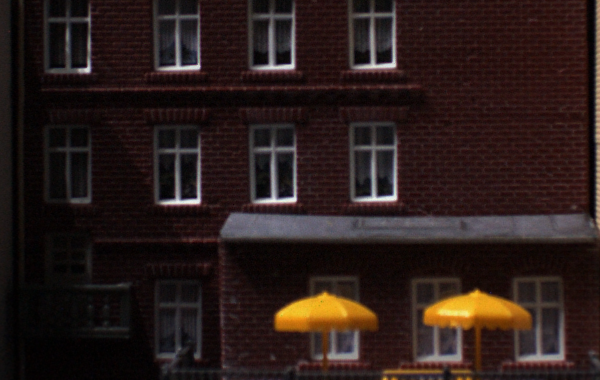
\includegraphics[width=\textwidth]{img/pixelNormalizationExample1.png}
        \caption{}
        \label{fig:pixelNormalizationExample1}
    \end{subfigure}
    \begin{subfigure}[t]{0.48\textwidth}
        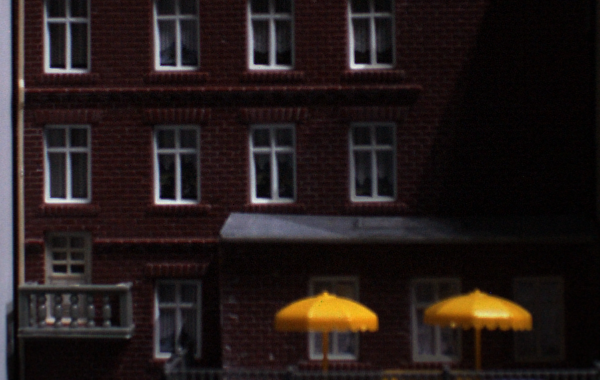
\includegraphics[width=\textwidth]{img/pixelNormalizationExample2.png}
        \caption{}
        \label{fig:pixelNormalizationExample2}
    \end{subfigure}
    \begin{subfigure}[t]{0.48\textwidth}
        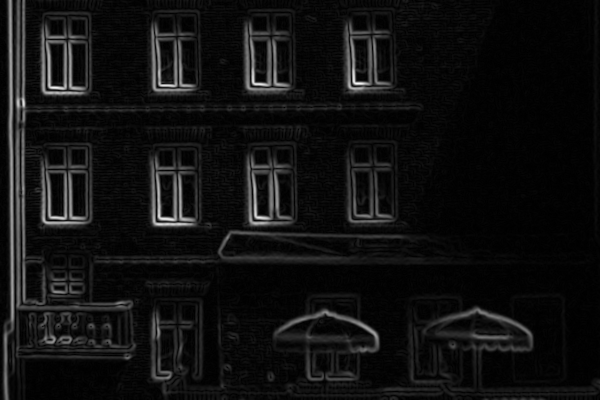
\includegraphics[width=\textwidth]{img/pixelNormalizationExample3.png}
        \caption{}
        \label{fig:pixelNormalizationExample3}
    \end{subfigure}
    \begin{subfigure}[t]{0.48\textwidth}
        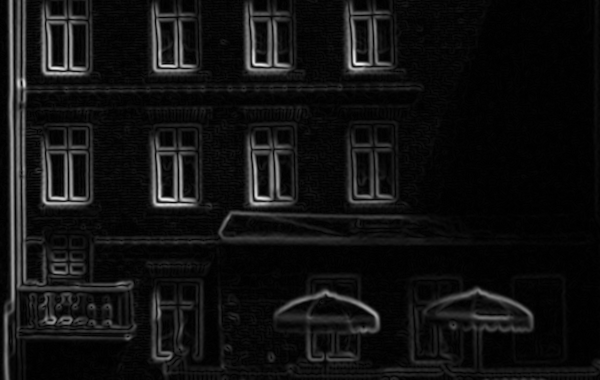
\includegraphics[width=\textwidth]{img/pixelNormalizationExample4.png}
        \caption{}
        \label{fig:pixelNormalizationExample4}
    \end{subfigure}
    \begin{subfigure}[t]{0.48\textwidth}
        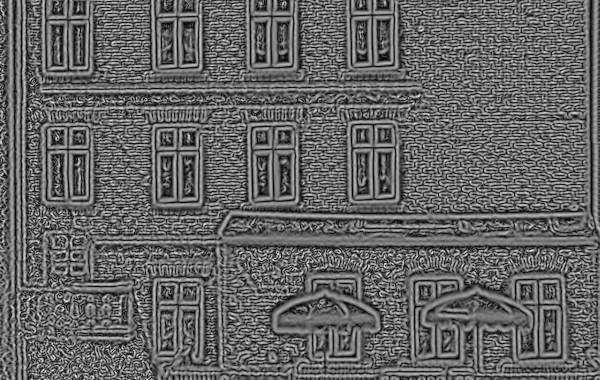
\includegraphics[width=\textwidth]{img/pixelNormalizationExample5.png}
        \caption{}
        \label{fig:pixelNormalizationExample5}
    \end{subfigure}
    \begin{subfigure}[t]{0.48\textwidth}
        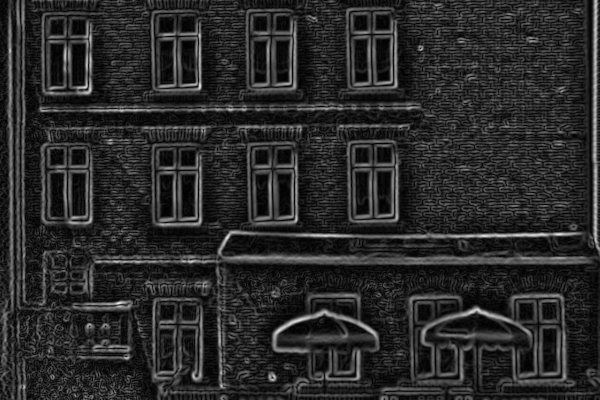
\includegraphics[width=\textwidth]{img/pixelNormalizationExample6.png}
        \caption{}
        \label{fig:pixelNormalizationExample6}
    \end{subfigure}
    \begin{subfigure}[t]{0.48\textwidth}
        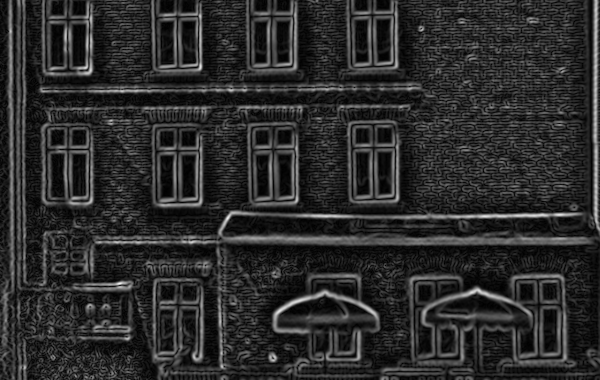
\includegraphics[width=\textwidth]{img/pixelNormalizationExample7.png}
        \caption{}
        \label{fig:pixelNormalizationExample7}
    \end{subfigure}
    \begin{subfigure}[t]{0.48\textwidth}
        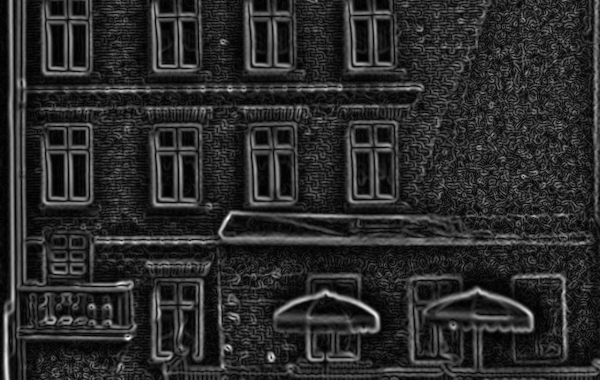
\includegraphics[width=\textwidth]{img/pixelNormalizationExample8.png}
        \caption{}
        \label{fig:pixelNormalizationExample8}
    \end{subfigure}
    \caption{Images \subref{fig:pixelNormalizationExample1} and \subref{fig:pixelNormalizationExample2} show cut-outs of an image with leftmost and rightmost artificial lighting, respectively. Images \subref{fig:pixelNormalizationExample3} and \subref{fig:pixelNormalizationExample4} show gradient magnitudes of these images. Images \subref{fig:pixelNormalizationExample5} and \subref{fig:pixelNormalizationExample6} show pixel normalized magnitudes for $\sigma_\text{norm} = 2$. Images \subref{fig:pixelNormalizationExample7} and \subref{fig:pixelNormalizationExample8} show pixel normalized magnitudes for $\sigma_\text{norm} = 10$.}
    \label{fig:pixelNormalizationExample}
\end{figure}
%
\section{Cell aperture function}
\label{sec:cellApertureFunction}
%
The purpose of the cell aperture functions $A_j$ is to weight points closer to each cell center higher in their respective cell histograms. We define a cell aperture function as a Gaussian function
%
\begin{align}
A_j(\x) = G(\x - \c_j; \sigmacellj)
\end{align}
%
where $\c_j$ is the cell center for cell $j$ and $\sigmacellj$ is the standard deviation of cell $j$.

The cell aperture function is defined for all cells in the feature. Having defined $A_j$ we are now able to define the \emph{grid layouts} that define the cell centers $\boldsymbol{c}_j$ for each feature. \Cref{fig:gridType} shows examples of the six different grid layouts that we propose for describing the local area around an interest point: polar, polar central, log-polar, concentric polar, concentric polar central, and concentric log-polar. These layouts are inspired by the GLOH \cite{mikolajczyk2005performance}, Irregular SIFT \cite{cui2009scale}, and DAISY \cite{tola2008fast} layouts. The four polar grids all rely on polar Gaussian aperture cell functions where $G$ is replaced by a polar Gaussian function converting the Cartesian coordinates into polar coordinates before applying the Gaussian function and converting back into Cartesian coordinates afterwards. The two log-polar grids both use Cartesian Gaussian aperture cell functions. The examples are shown for the \emph{grid size} $8\times 2$ meaning that each layout has 8 cells in each of their 2 rings. The two ``central'' and log-polar grids additionally have a single central cell.

All these layouts are defined relative to the \emph{grid radius}, which is defined as a constant times the detection scale of the feature. In other words the grid radius defines the span of the feature. The grid layouts are defined such that by default the 1 standard deviation curves of the outer-most cells in the feature touch the grid radius. Each ring consists of $n$ cells dividing the ring equally in the angular direction. Furthermore the following holds for each of the specific layouts:

For log-polar layouts the radial span of each ring is defined such that the 1 standard deviation curve $\sigmacellj$ of a cell $j$ touches the 1 standard deviation curves of the neighbouring rings and neighbouring angles by default. This results in different default cell sigmas for the normal and concentric log-polar grid layouts since the concentric log-polar grid layout can pack the cells more densely without overlapping cells as seen in \Cref{fig:gridTypeLp,fig:gridTypeClp}.

For polar layouts the radial span is divided equally between the rings. The polar central layouts are furthermore having a central cell of half the radial span of the rings. The polar Gaussian cell aperture function combined with postioning of the cell centers $\c_j$ are shown in \Cref{fig:gridTypeP,fig:gridTypePc,fig:gridTypeCp,fig:gridTypeCpc}.
See \Cref{apx:gridLayouts} for more information on how to compute the grid layout positions.

As mentioned in the descriptions above, the grids are defined with default cell sigmas. All these cell sigmas can be scaled both up and down to allow for additional or less overlap between the cells. This will however not change the positioning of the cell centers $\c_j$.

For the grid layout examples in this section, we have simply chosen a grid size and a grid radius. These two variables are however having a major impact on the dimensionality and final outcome of the descriptor along with $\sigmacellj$, and hence these three parameters are tuned in our parameter studies in order to get the optimal descriptor layout and overlap.

\Cref{fig:gridTypeWindow} shows examples of the two grid layouts that we propose for describing sliding windows, where we wish to have a more uniform description across the whole window. Following the same logic as before, we construct the grids such that by default the 1 standard deviation curves of neighbouring cells are tangent to each other, and allow a scaling of these by $\sigmacellj$.

\begin{figure}[p]
	\centering
	\begin{subfigure}[t]{\textwidth}
		\centering
		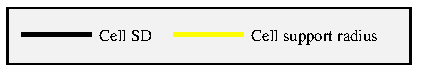
\includegraphics[width=0.5\textwidth]{img/cellWindow_legend.pdf}
	\end{subfigure}
	\begin{subfigure}[t]{0.40\textwidth}
		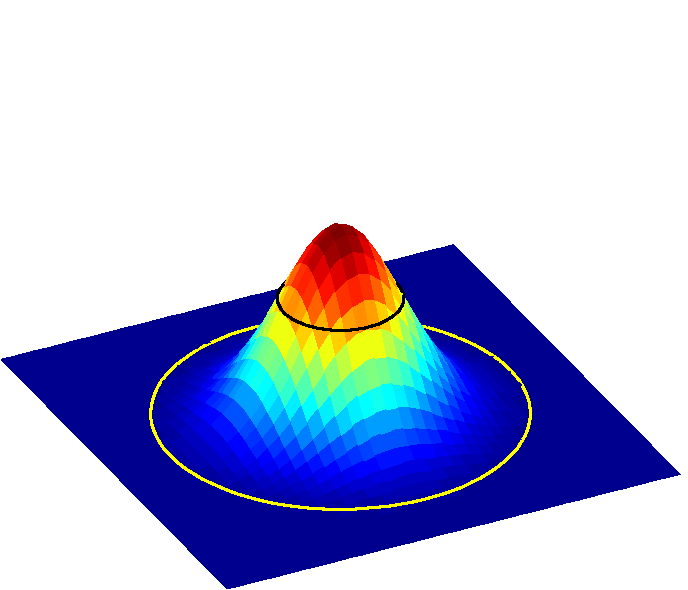
\includegraphics[width=\textwidth, clip=true, trim=0 0 0 90]{img/cellWindow.pdf}
		\caption{Gaussian}
		\label{fig:cellWindow}
	\end{subfigure}
	\begin{subfigure}[t]{0.40\textwidth}
		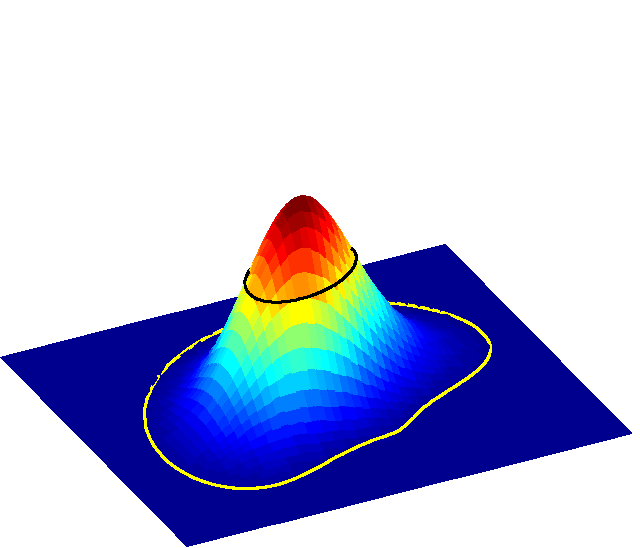
\includegraphics[width=\textwidth, clip=true, trim=0 0 0 90]{img/cellWindowPolar.pdf}
		\caption{Polar Gaussian}
		\label{fig:cellWindowPolar}
	\end{subfigure}
	\caption{The two types of Gaussian cell aperture functions plotted in 3-D. The black curves are placed 1 standard deviation $\sigma$ from the cell centers. The yellow curves are placed $3 \sigma$ from the cell centers and confine the regions used to calculate the cell histograms.}
	\label{fig:gridWindow}
	\vspace{2mm}
	\begin{subfigure}[t]{\textwidth}
		\centering
		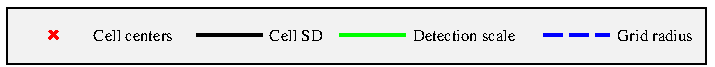
\includegraphics[width=\textwidth]{img/gridType_legend.pdf}
	\end{subfigure}
	\begin{subfigure}[t]{0.30\textwidth}
		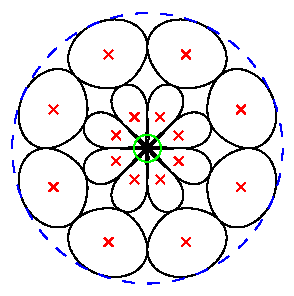
\includegraphics[width=\textwidth]{img/gridType_polar_polar_gaussian.pdf}
		\caption{Polar}
		\label{fig:gridTypeP}
	\end{subfigure}
	\begin{subfigure}[t]{0.30\textwidth}
		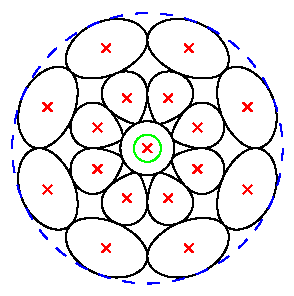
\includegraphics[width=\textwidth]{img/gridType_polar_central_polar_gaussian.pdf}
		\caption{Polar central}
		\label{fig:gridTypePc}
	\end{subfigure}
	\begin{subfigure}[t]{0.30\textwidth}
		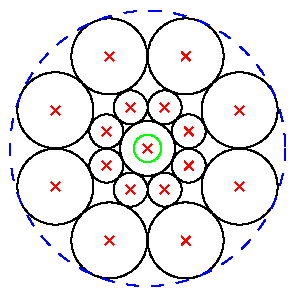
\includegraphics[width=\textwidth]{img/gridType_log-polar.pdf}
		\caption{Log-polar}
		\label{fig:gridTypeLp}
	\end{subfigure}
	\begin{subfigure}[t]{0.30\textwidth}
		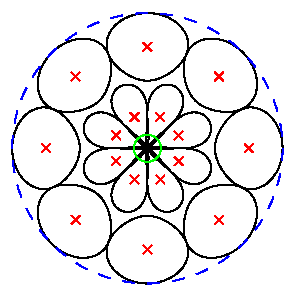
\includegraphics[width=\textwidth]{img/gridType_concentric_polar_polar_gaussian.pdf}
		\caption{Concentric polar}
		\label{fig:gridTypeCp}
	\end{subfigure}
	\begin{subfigure}[t]{0.30\textwidth}
		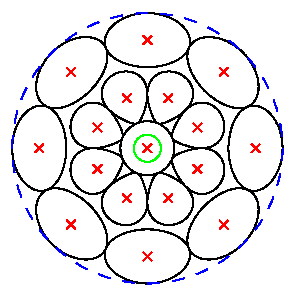
\includegraphics[width=\textwidth]{img/gridType_concentric_polar_central_polar_gaussian.pdf}
		\caption{\footnotesize Concentric polar central}
		\label{fig:gridTypeCpc}
	\end{subfigure}
	\begin{subfigure}[t]{0.30\textwidth}
		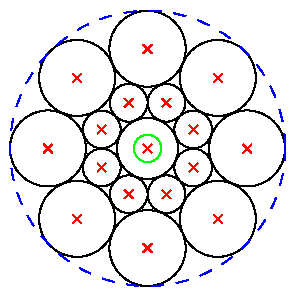
\includegraphics[width=\textwidth]{img/gridType_concentric_log-polar.pdf}
		\caption{Concentric log-polar}
		\label{fig:gridTypeClp}
	\end{subfigure}
	\caption{Examples of grid layouts centered around a detected interest point, showing cell centers, 1 standard deviation curves (see \Cref{fig:gridWindow}), detection scales, and grid radii. The grid size is chosen to be $8 \times 2$ (8 cells in each of 2 rings) and the grid radius is set to 10 times detection scale. The polar grids utilize polar Gaussian aperture cell functions while the log-polar use Cartesian Gaussian aperture cell functions.}
	\label{fig:gridType}
\end{figure}
%
\begin{figure}
	\centering
	\begin{subfigure}[t]{\textwidth}
		\centering
		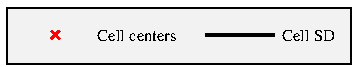
\includegraphics[width=0.5\textwidth]{img/gridType_legend_cropped.pdf}
	\end{subfigure}
	\begin{subfigure}[t]{0.45\textwidth}
		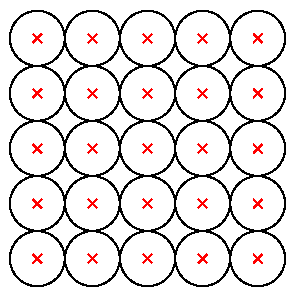
\includegraphics[width=\textwidth]{img/gridType_square_window.pdf}
		\caption{Square grid}
		\label{fig:gridTypeSquare}
	\end{subfigure}
	\begin{subfigure}[t]{0.45\textwidth}
		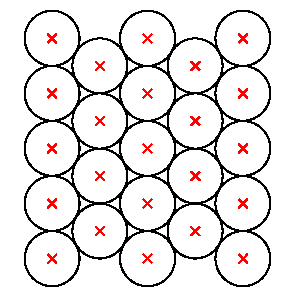
\includegraphics[width=\textwidth]{img/gridType_triangle_window.pdf}
		\caption{Triangular grid}
		\label{fig:gridTypeTriangle}
	\end{subfigure}
	\caption{Examples of grid layouts used for sliding windows, where we are interested in describing a larger area rather than the local area surrounding a detected point.}
\label{fig:gridTypeWindow}
\end{figure}
%
\section{Center aperture function}
\label{sec:centerApertureFunction}
%
Similarly to $A_j$, the purpose of the center aperture function $P$ is to weight points closer to the detected interest point higher, since they are of greater importance to the local structure. We define it as a Gaussian function
%
\begin{align}
P(\x) = G(\x - \p; \sigmacenter)
\end{align}
%
where $\p$ is the interest point and $\sigmacenter$ is the standard deviation of the center aperture function. The $\sigmacenter$ is by default equal to the grid radius but can be scaled both up and down to achieve the best performance. The center aperture function is inspired by SIFT \cite{lowe2004distinctive} and DAISY \cite{tola2008fast} which similarly use a center aperture function. For SIFT the standard deviation of the corresponding function is however pre-defined to have a $\sigma$ 1.5 times its square-grid width and height, whereas we choose to find the optimal $\sigmacenter$ by adding it to our parameterstudies.
%
\section{Binning aperture function}
%
As mentioned in the introduction to the proposed descriptor, we use smooth histograms as described in \Cref{sec:histograms} for our descriptor. The binning aperture function decides the shape of the smooth histograms that make up our descriptor. We define it as a Gaussian function
\begin{align}
	B(f_i, \x; f) = G(f(\x) - f_i; \sigma)
\end{align}

For our proposed descriptor value function $f$ is either the gradient orientation or the shape index. The number $n_\text{bins}$ of bin centers $f_i$ for $i = 1,\hdots,n_\text{bins}$ is variable and hence we need to define the bin centers as a function of $n_\text{bins}$. Given an interval $[a,b]$, we define the bin centers $f_i$
\begin{align}
	\label{eq:binCenters}
	f_i &= a + \frac{b-a}{n_\text{bins}} \left(i - \frac{1}{2} \right)
\end{align}
which corresponds to splitting the interval into $n_\text{bins}$ equally sized parts and placing the bin centers $f_i$ in each of the $n_\text{bins}$ centers of these parts.

The shape index has values spanning the interval $[-1,1]$, and hence by placing the bin centers according to \Cref{eq:binCenters} their areas will integrate to different values. This is handled by integrating the area and re-normalizing by this value for each bin center. The integration is performed as described in \Cref{sec:histogramsGaussianFilter}. The gradient orientation has values spanning the periodic interval $[-\pi,\pi]$. Since the interval is periodic, all bin centers integrate to the same area and hence we choose to omit re-normalization when computing the gradient orientation to save computations. The perodicity is implemented by using simple wrap-around of the distance $f(\x) - f_i$.
%
\subsection{Histogram normalization}
We have now covered all the functions needed in order to compute the $j$'th histogram $H_j$, \Cref{eq:proposed_histogram}, for each cell $j$ as well as the positioning of each of these cells. The last operation we need to perform to get our descriptor $D$, \Cref{eq:proposed_descriptor}, is a concatenation of all the $H_j$ histograms. Finally we view $D$ as a single vector and normalize it by using the $L_2$-norm as \citet{lowe2004distinctive} does in his SIFT descriptor. This could cause problems when dealing with occluded interest points and hence other strategies could be persued. We have however not chosen to do so.\todo{Decide whether to persue other strategies or not}
%
\section{Example}
%
In order to visualize the construction of our descriptor, we will show an example of the whole process. As value and magnitude functions we choose the standard gradient orientation with gradient magnitude. We start by extracting interest points from an image with a multi-scale DoG detector, as shown in \Cref{fig:cellHistDetector}.

The next step is to construct the scale space images as described in \Cref{sec:valueMagnitudeFunctions} based on the DoG scales. This results in scale space images which are smoothed and downsampled versions of the original image. Both operations are done according to the respective scales, which causes all features to have the same size in pixels regardless of their respective scales. We compute the new feature coordinates in the scale space images, and remove those points that are too close to the edge: if any cell support radius (shown in \Cref{fig:gridWindow}) belonging to a feature would span outside the image border, we discard the feature. \Cref{fig:cellHistScaleSpacesP} shows a handful of these images with their respective features, and which of these are discarded.

\begin{figure}[p]
    \centering
    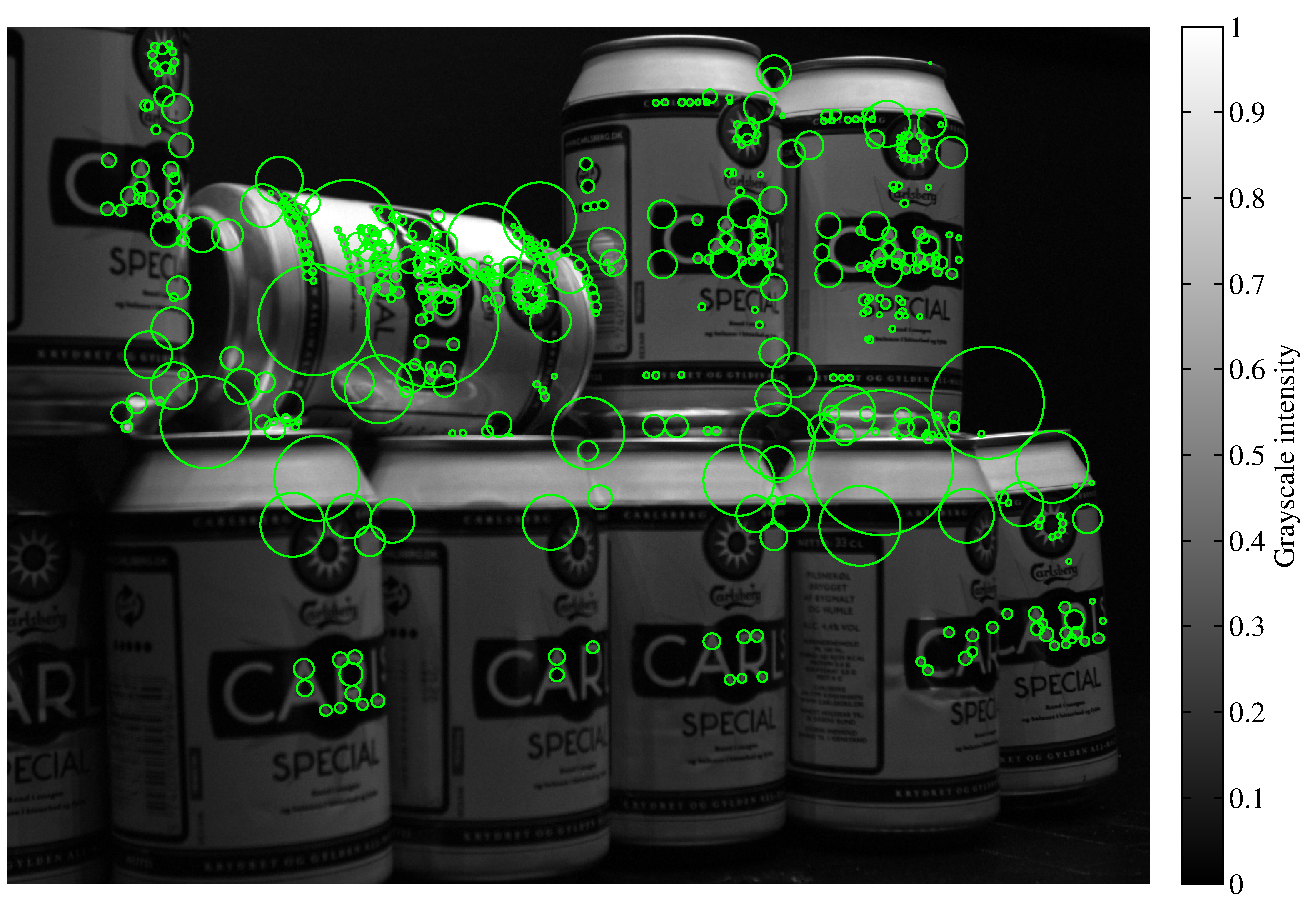
\includegraphics[width=\textwidth]{img/cellHistDetector.pdf}
    \caption{Interest points (green) found by a multi-scale DoG detector on an example image. The circle radii illustrate the detection scale of each point. $529$ points are detected in total.}
    \label{fig:cellHistDetector}
    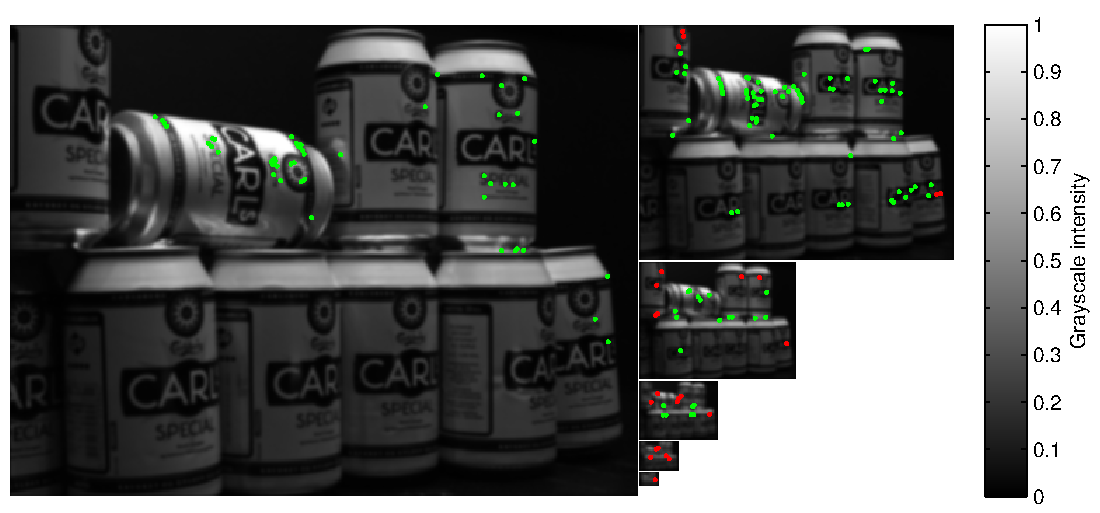
\includegraphics[width=\textwidth]{img/cellHistScaleSpacesP.pdf}
    \caption{The smoothed and downsampled images at various scales with their corresponding kept interest points (green) and removed interest points (red).}
    \label{fig:cellHistScaleSpacesP}
\end{figure}

\begin{figure}[p]
    \centering
    \begin{subfigure}[t]{0.97\textwidth}
		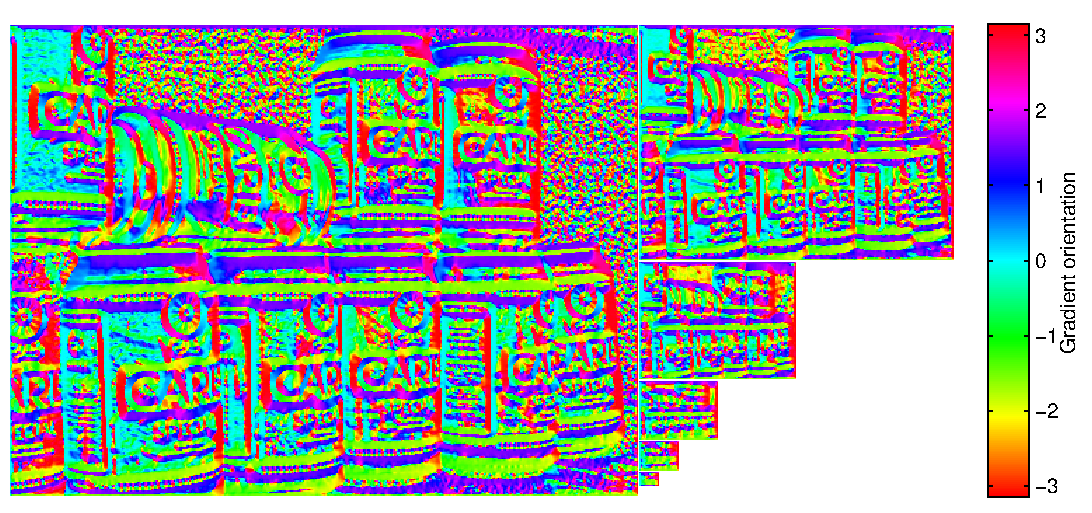
\includegraphics[width=\textwidth]{img/cellHistScaleSpacesV.pdf}
    	\caption{Gradient orientation images}
    	\label{fig:cellHistScaleSpacesV}
	\end{subfigure}
    \begin{subfigure}[t]{0.97\textwidth}
		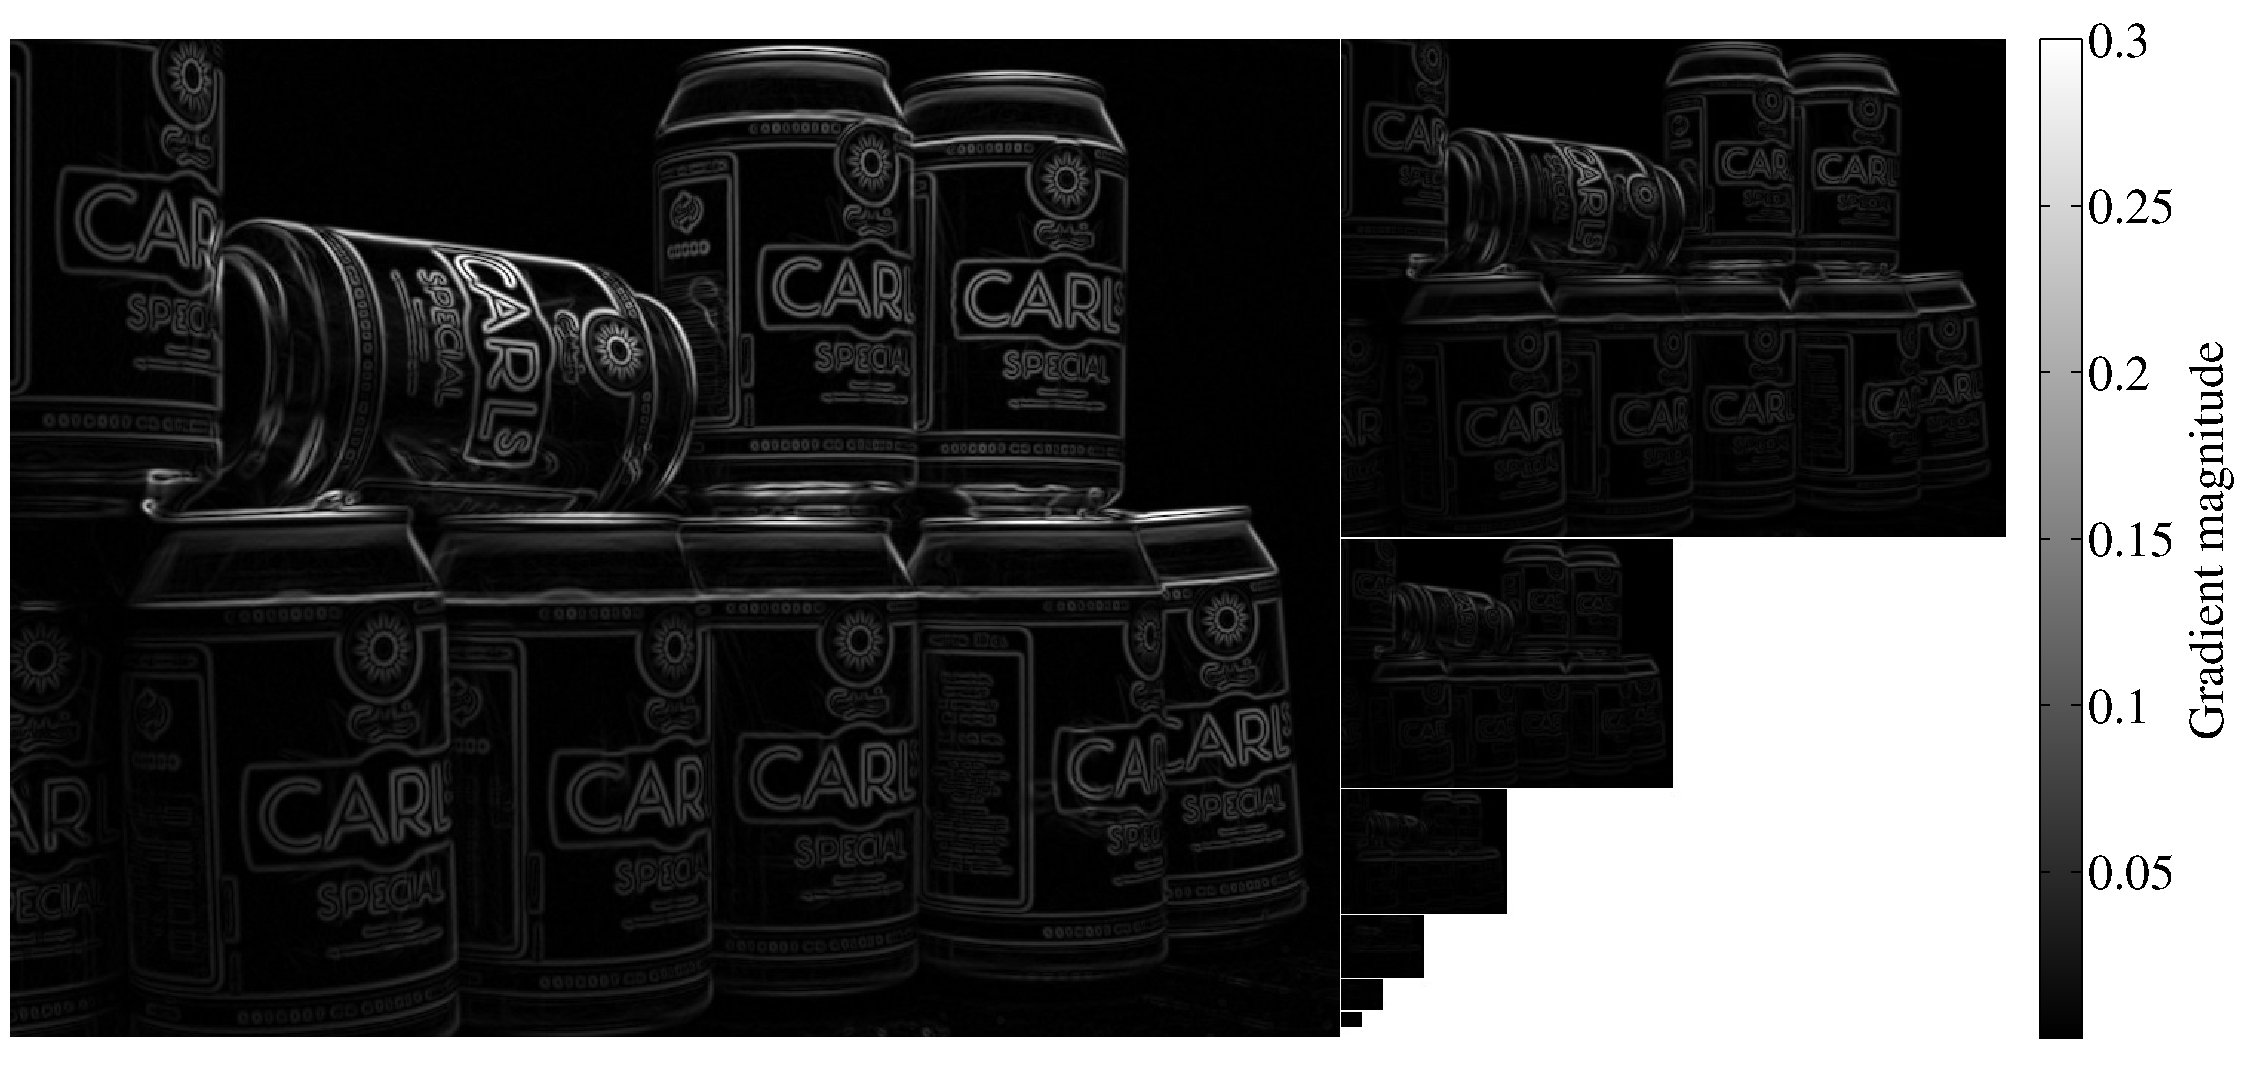
\includegraphics[width=\textwidth]{img/cellHistScaleSpacesM.pdf}
    	\caption{Gradient magnitude images}
    	\label{fig:cellHistScaleSpacesM}
	\end{subfigure}
	\begin{subfigure}[t]{0.97\textwidth}
		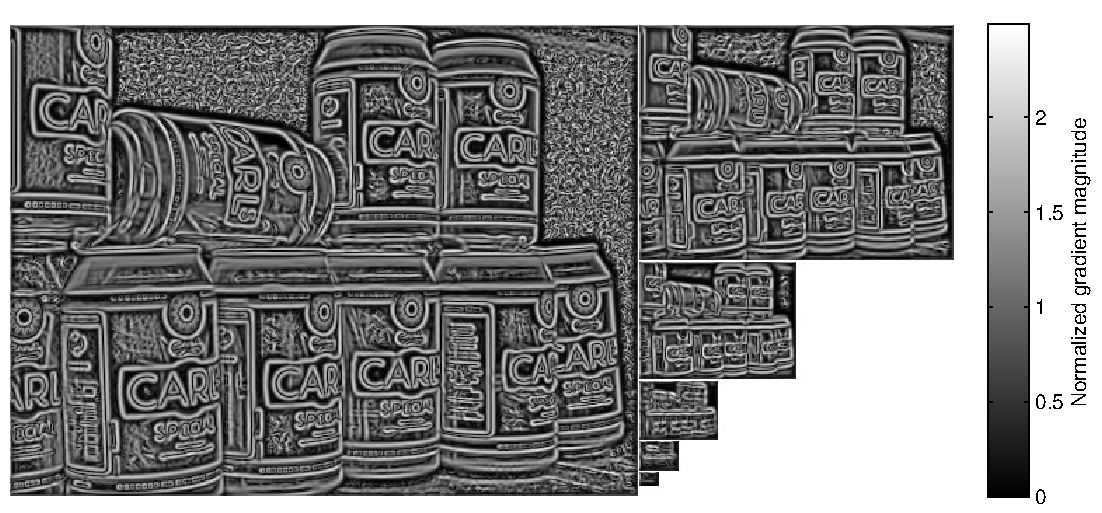
\includegraphics[width=\textwidth]{img/cellHistScaleSpacesMnorm.pdf}
    	\caption{Normalized pixel magnitude images}
    	\label{fig:cellHistScaleSpacesMnorm}
	\end{subfigure}
	\caption{Images \subref{fig:cellHistScaleSpacesV} and \subref{fig:cellHistScaleSpacesM} show gradient orientation and magnitude images computed at various scales. Image \subref{fig:cellHistScaleSpacesMnorm} shows the pixel normalized magnitude images, where the magnitudes are relative to a small local area.}
	\label{fig:cellHistScaleSpacesVM}
\end{figure}

\begin{figure}[p]
    \centering
    \begin{subfigure}[t]{0.97\textwidth}
		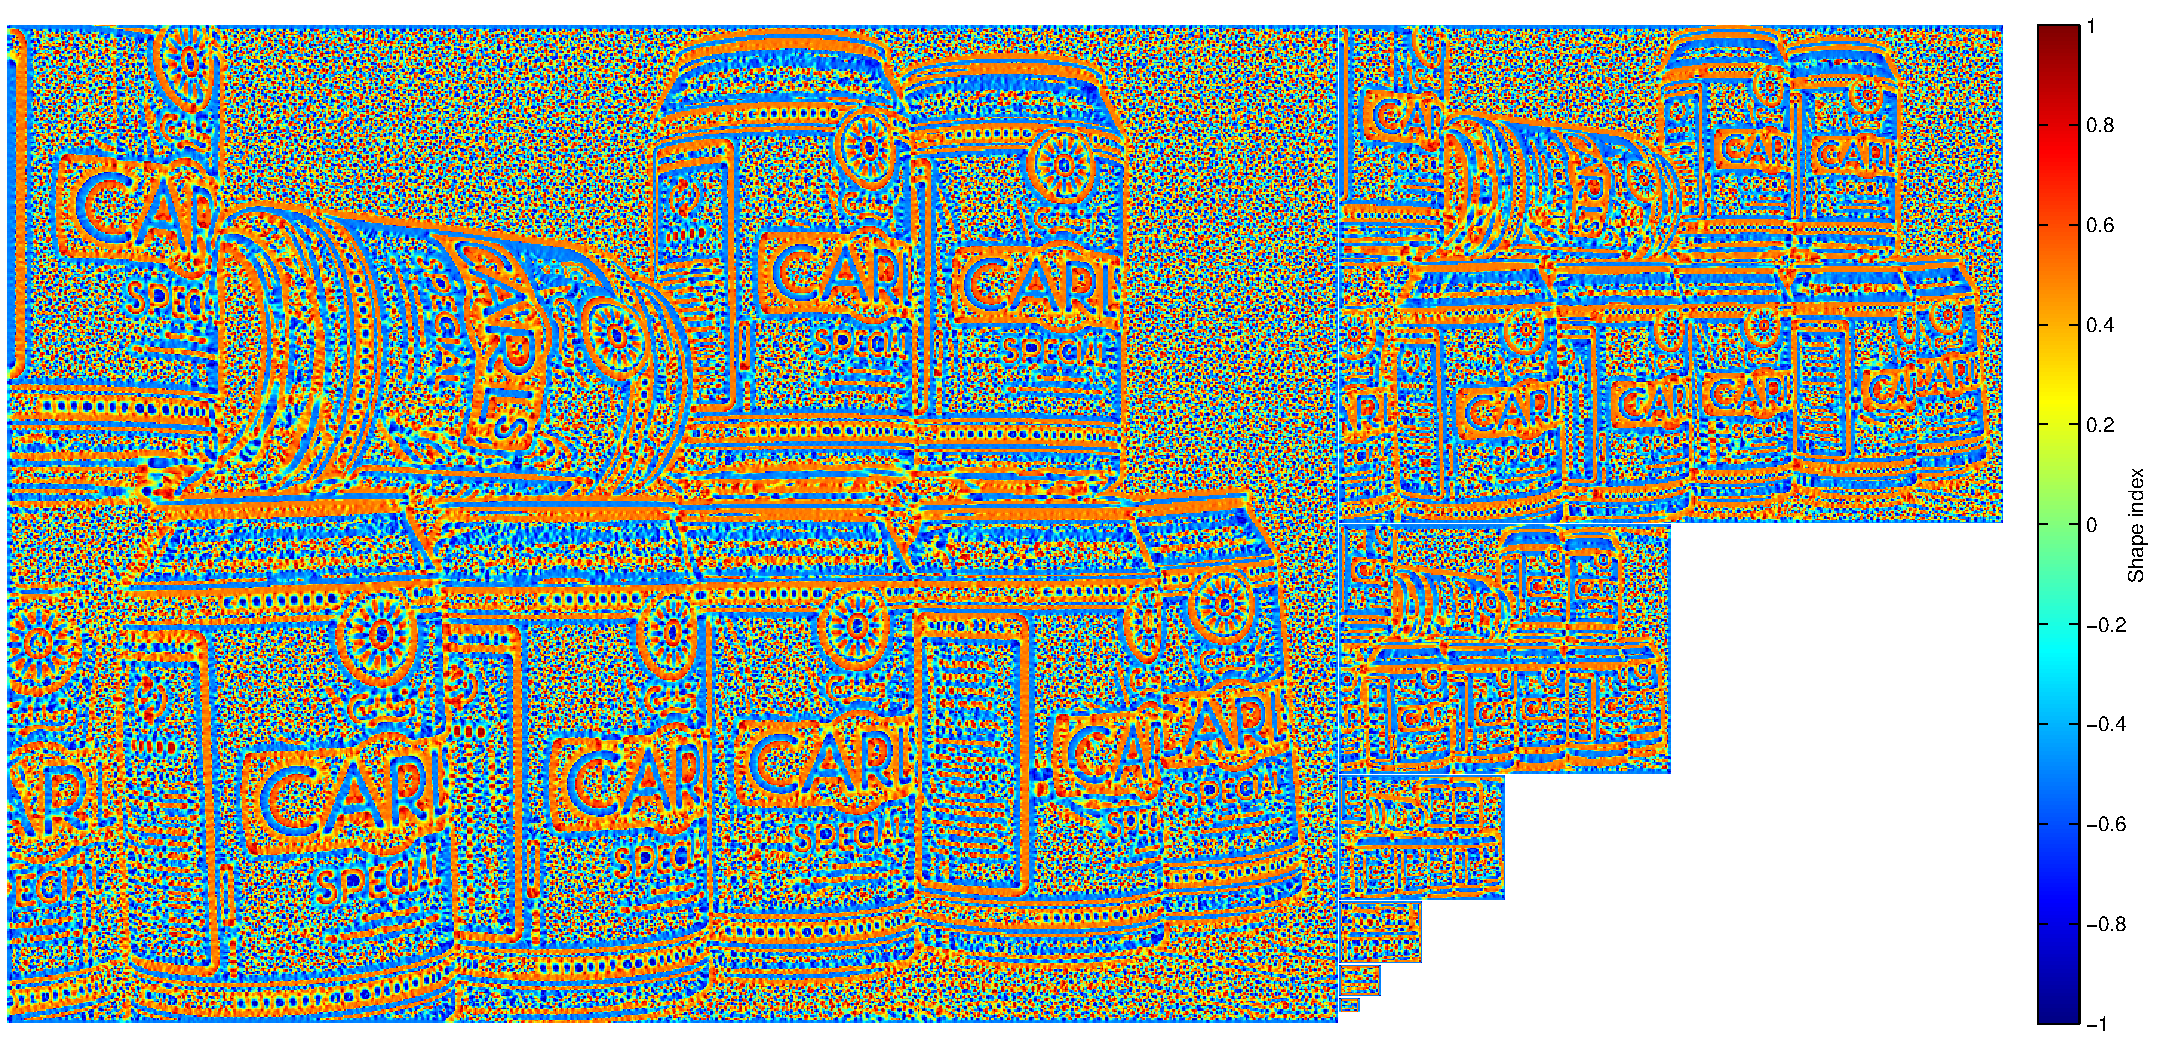
\includegraphics[width=\textwidth]{img/cellHistScaleSpacesS.pdf}
    	\caption{Shape index images}
    	\label{fig:cellHistScaleSpacesS}
	\end{subfigure}
    \begin{subfigure}[t]{0.97\textwidth}
		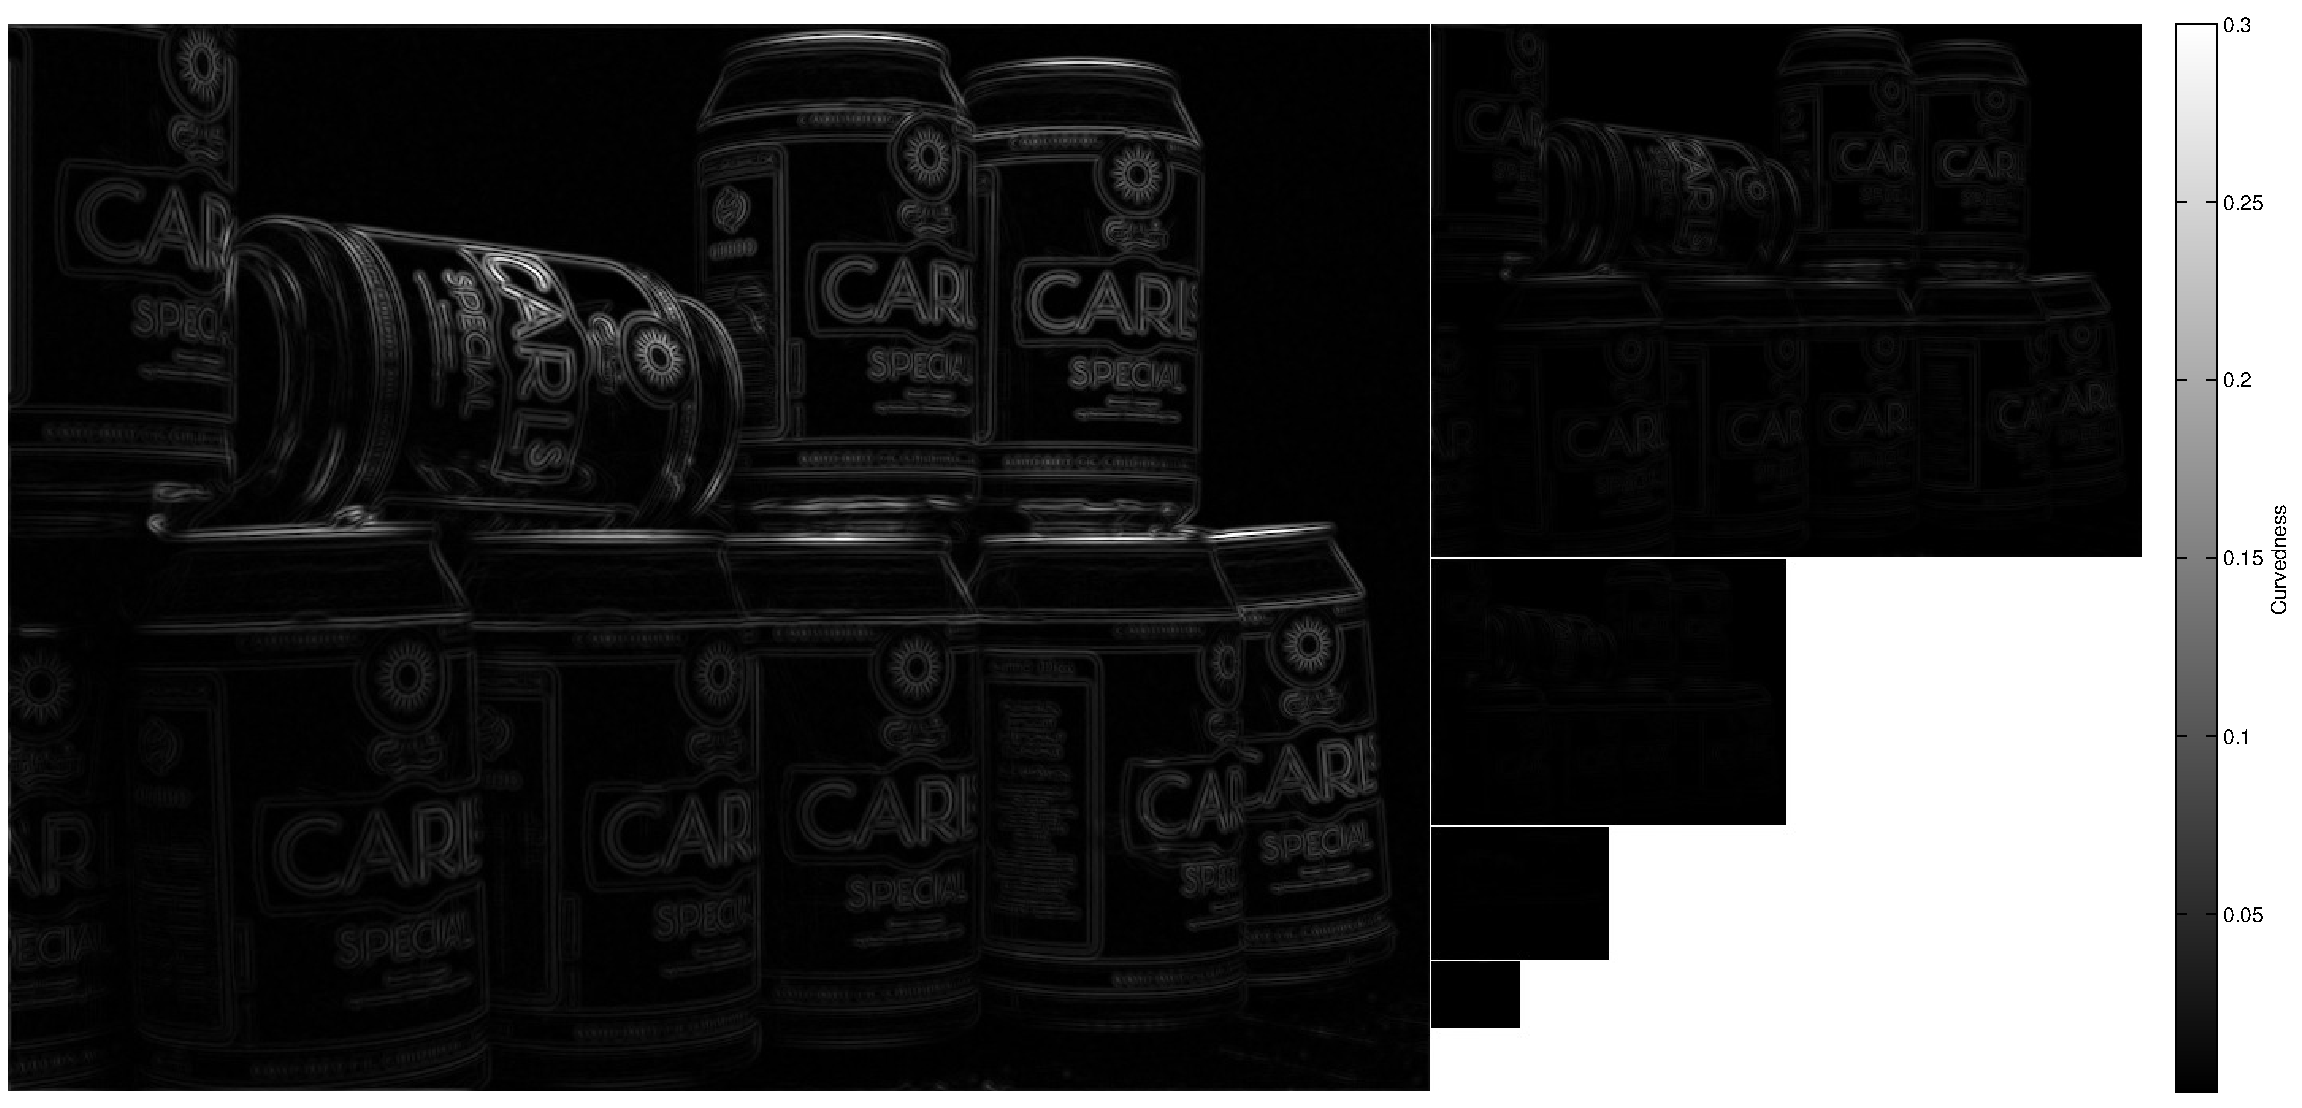
\includegraphics[width=\textwidth]{img/cellHistScaleSpacesC.pdf}
    	\caption{Curvedness images}
    	\label{fig:cellHistScaleSpacesC}
	\end{subfigure}
	\begin{subfigure}[t]{0.97\textwidth}
		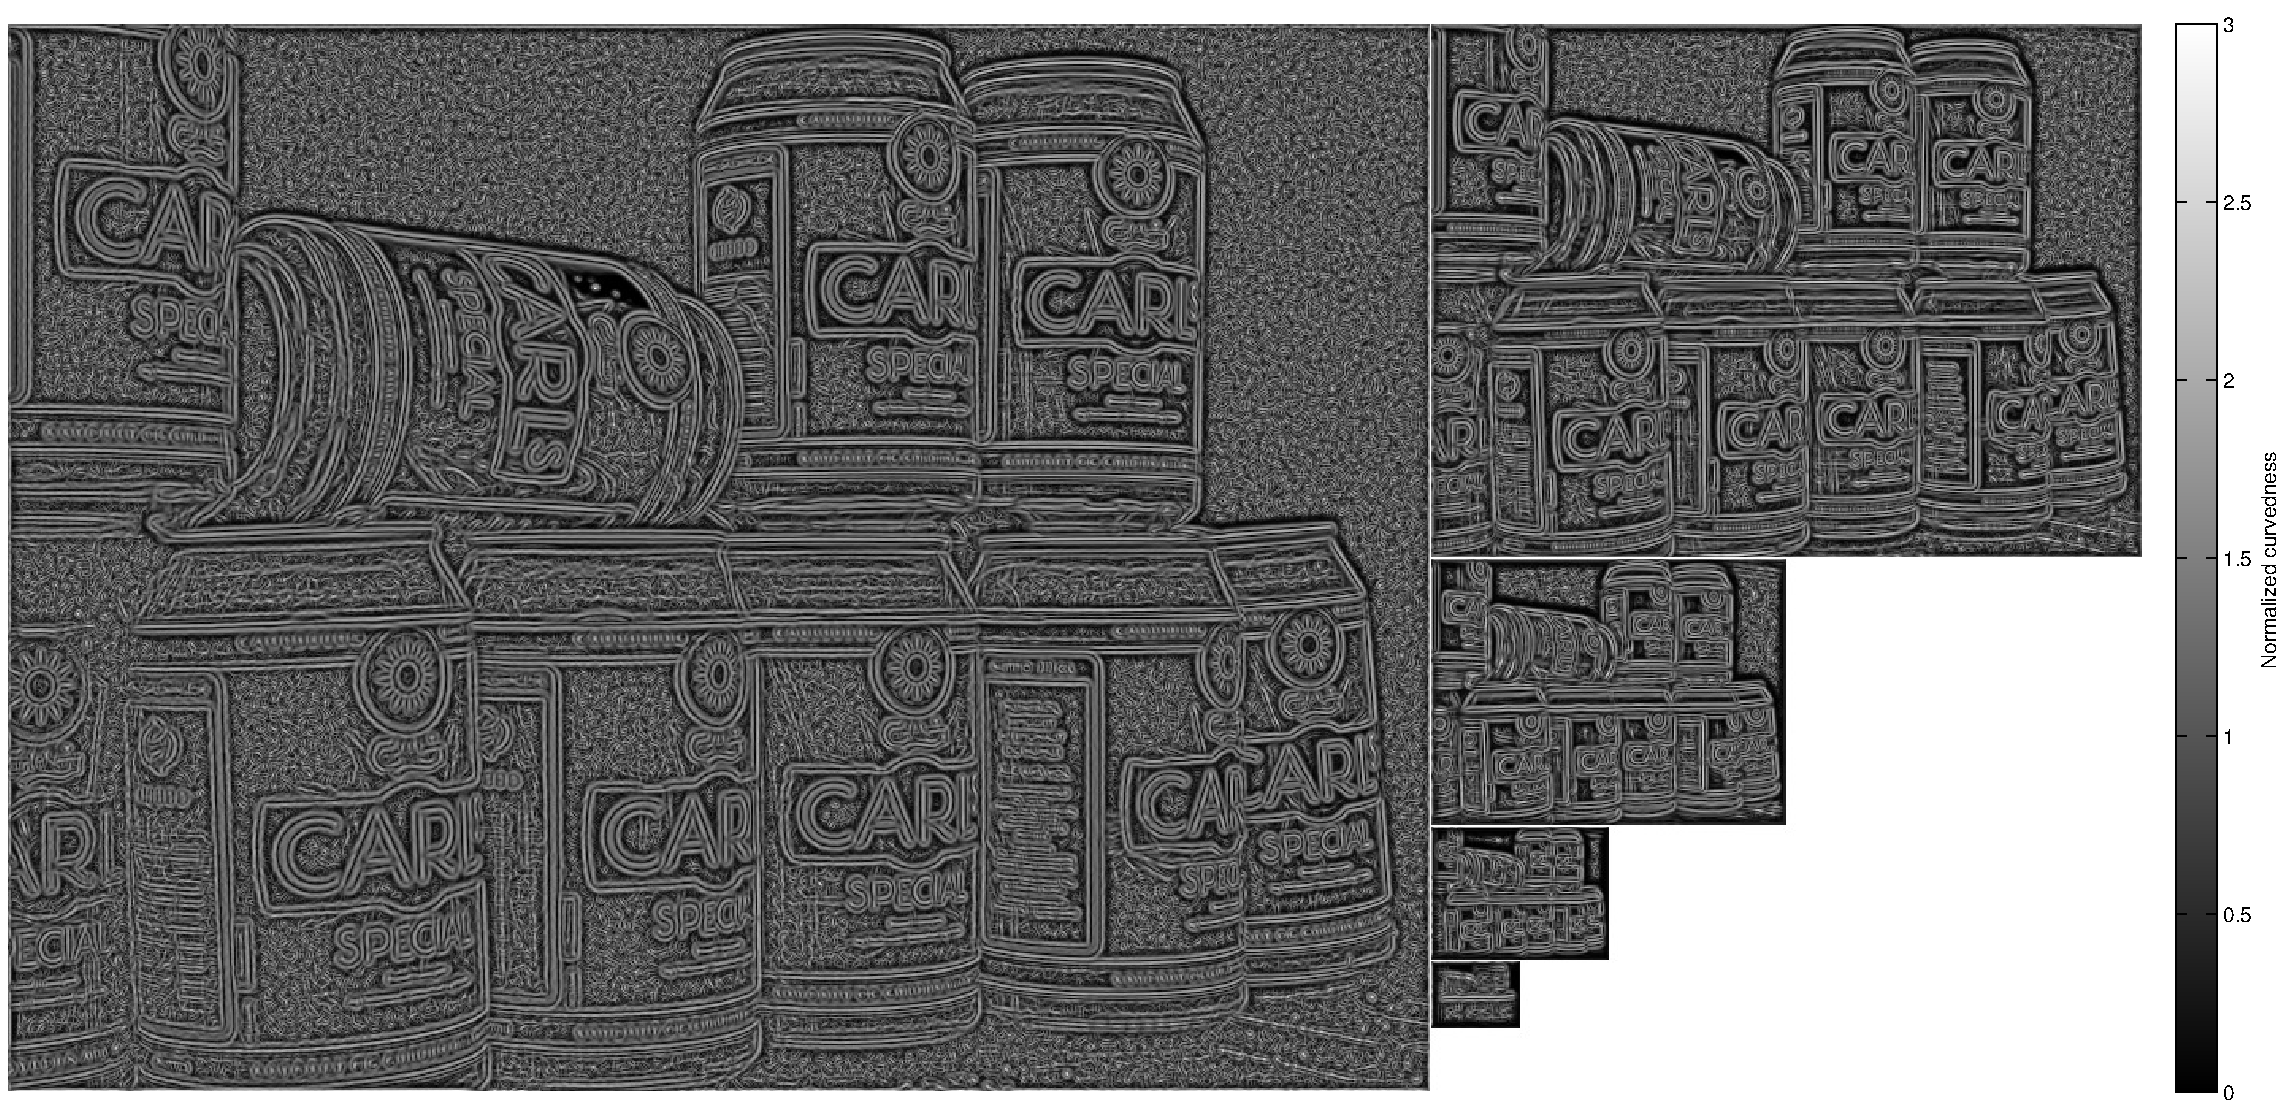
\includegraphics[width=\textwidth]{img/cellHistScaleSpacesCnorm.pdf}
    	\caption{Normalized curvedness images}
    	\label{fig:cellHistScaleSpacesCnorm}
	\end{subfigure}
	\caption{Images \subref{fig:cellHistScaleSpacesS} and \subref{fig:cellHistScaleSpacesC} show shape index and curvedness images computed at various scales. Image \subref{fig:cellHistScaleSpacesCnorm} shows the pixel normalized curvedness images, where the curvedness is relative to a small local area.}
	\label{fig:cellHistScaleSpacesSC}
\end{figure}

From the blurred and downsampled images we apply derivative filters in order to compute value and magnitude images by their respective functions. In this case only $x$ and $y$-derivatives are needed, which are used to compute gradient orientation and magnitude images. We then apply our pixel normalization scheme to the magnitudes. These images are shown in \Cref{fig:cellHistScaleSpacesVM}.

We need to compute the cell and center weights for pixels in every cell according to the chosen grid layout parameters. In order to save computation time, we confine the support radius of the Gaussian cell aperture filters to $3 \sigmacellj$, ignoring pixels outside this distance to each cell center. For pixels inside, we compute the spatial weights according to \Cref{sec:cellApertureFunction,sec:centerApertureFunction}. The products of these weights are illustrated in \Cref{fig:cellHistScaleSpacesSpatialWeights}, though since many cells overlap we show the maximal weight for each pixel.
The last type of weights needed are the bin values. \Cref{fig:cellHistScaleSpacesBins} shows bin value images for two bin centers with opposite gradient orientations. The images clearly show their corresponding parts of the beer can structures as well as some background noise. Though not shown in these images, to save computation time we only compute bin values once for each pixel with a non-zero spatial weight, and then simply look up the value when needed in a cell.


Finally the four weights are multiplied in order to construct the cell histograms. \Cref{fig:cellHistFigureGoM} illustrates one grid of these for a single feature. We see that there is a correspondence between the dominating orientations of the histograms and the gradient field of the underlying image. The weighted histogram values are then concatenated and normalized for each feature, resulting in the final descriptor.

\begin{figure}[tb]
    \centering
    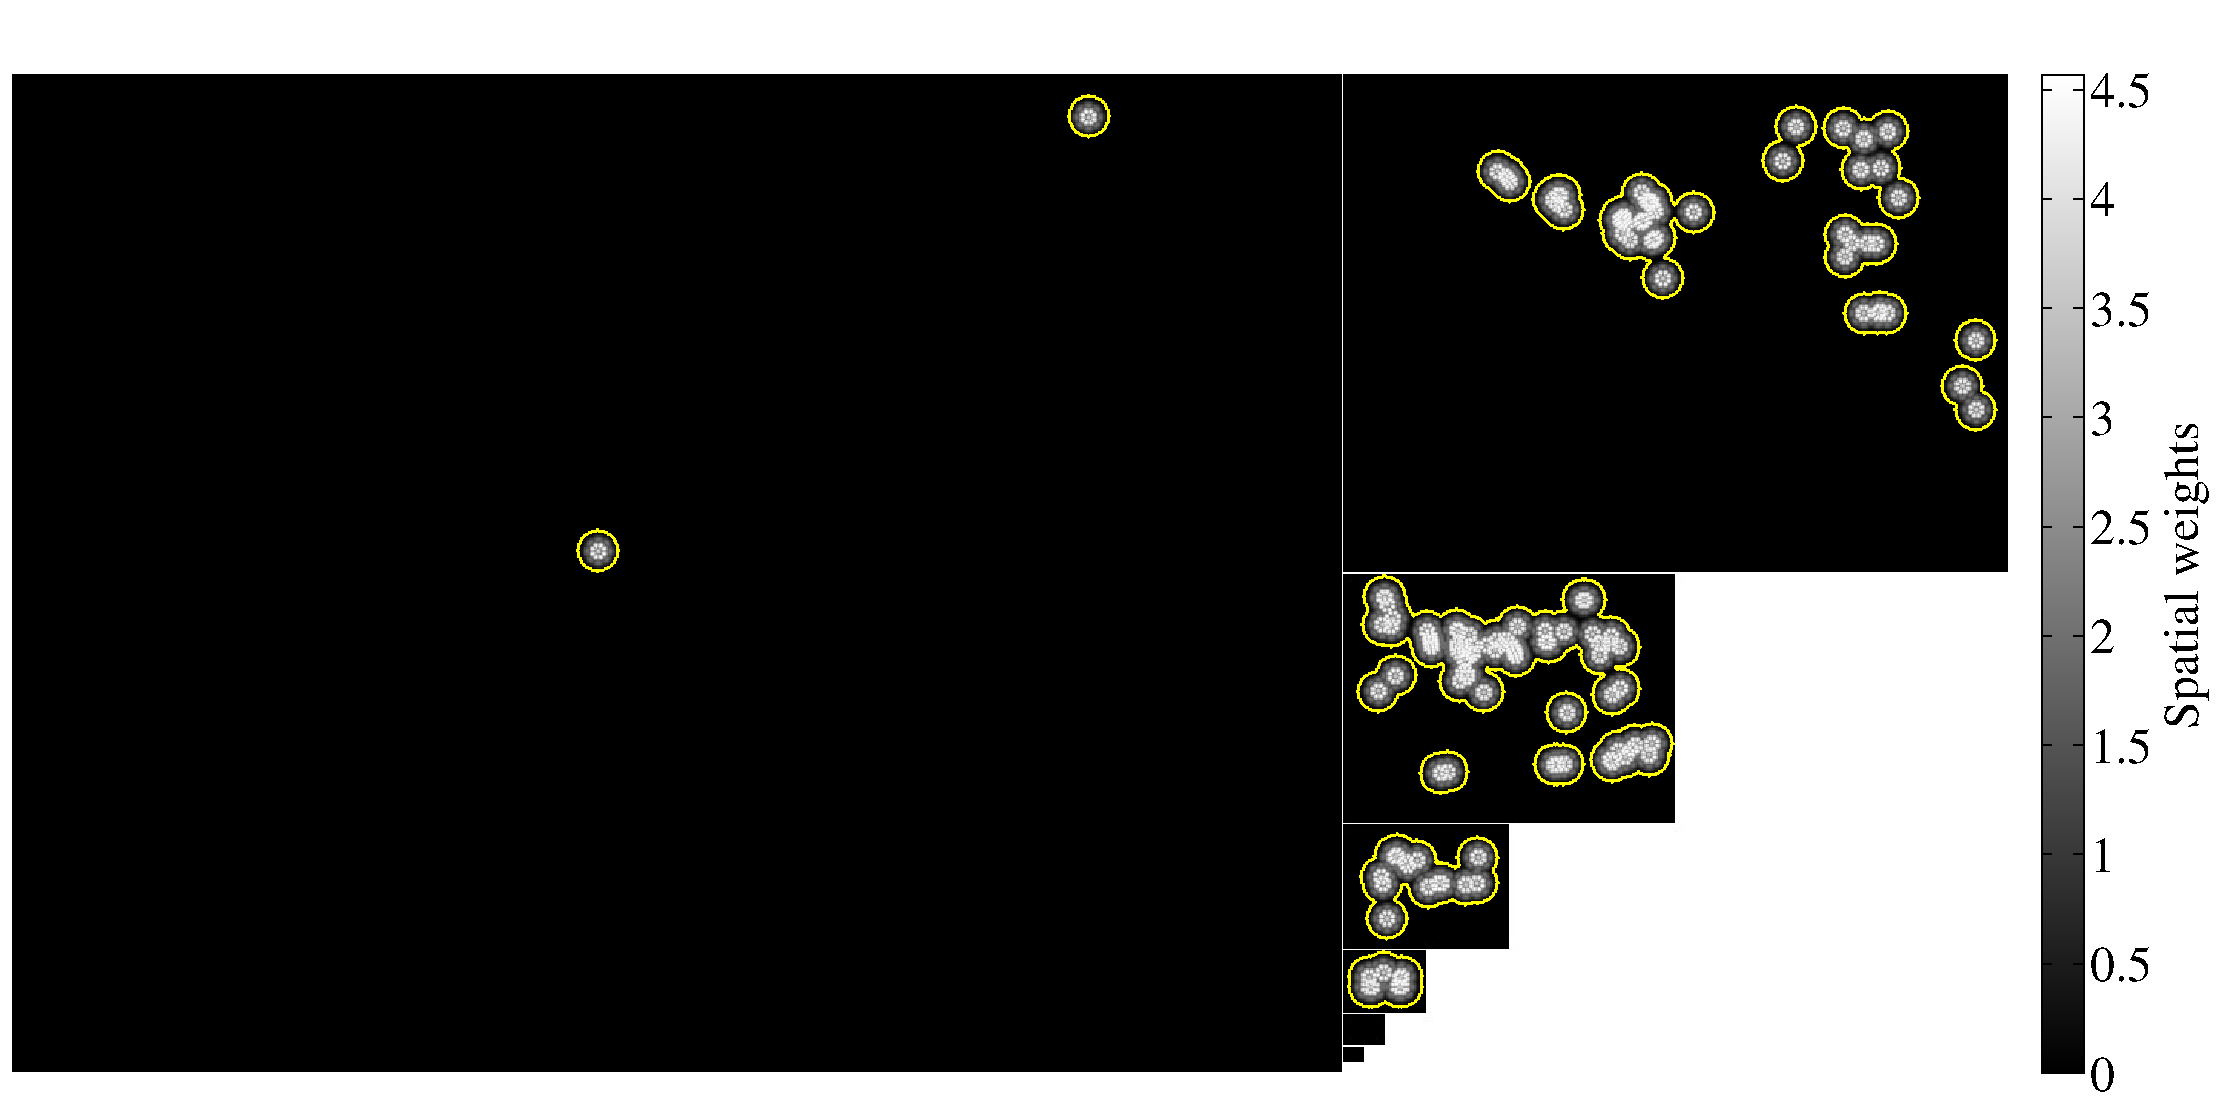
\includegraphics[width=\textwidth]{img/cellHistScaleSpacesSpatialWeights.pdf}
    \caption{Product of cell and center weights. When cells overlap, the maximal weight is shown. The yellow borders indicate the scope of pixels within the support radii of the cells. Only these are used to construct the cell histograms.}
    \label{fig:cellHistScaleSpacesSpatialWeights}
\end{figure}

\begin{figure}[p]
	\centering
	\begin{subfigure}[t]{\textwidth}
		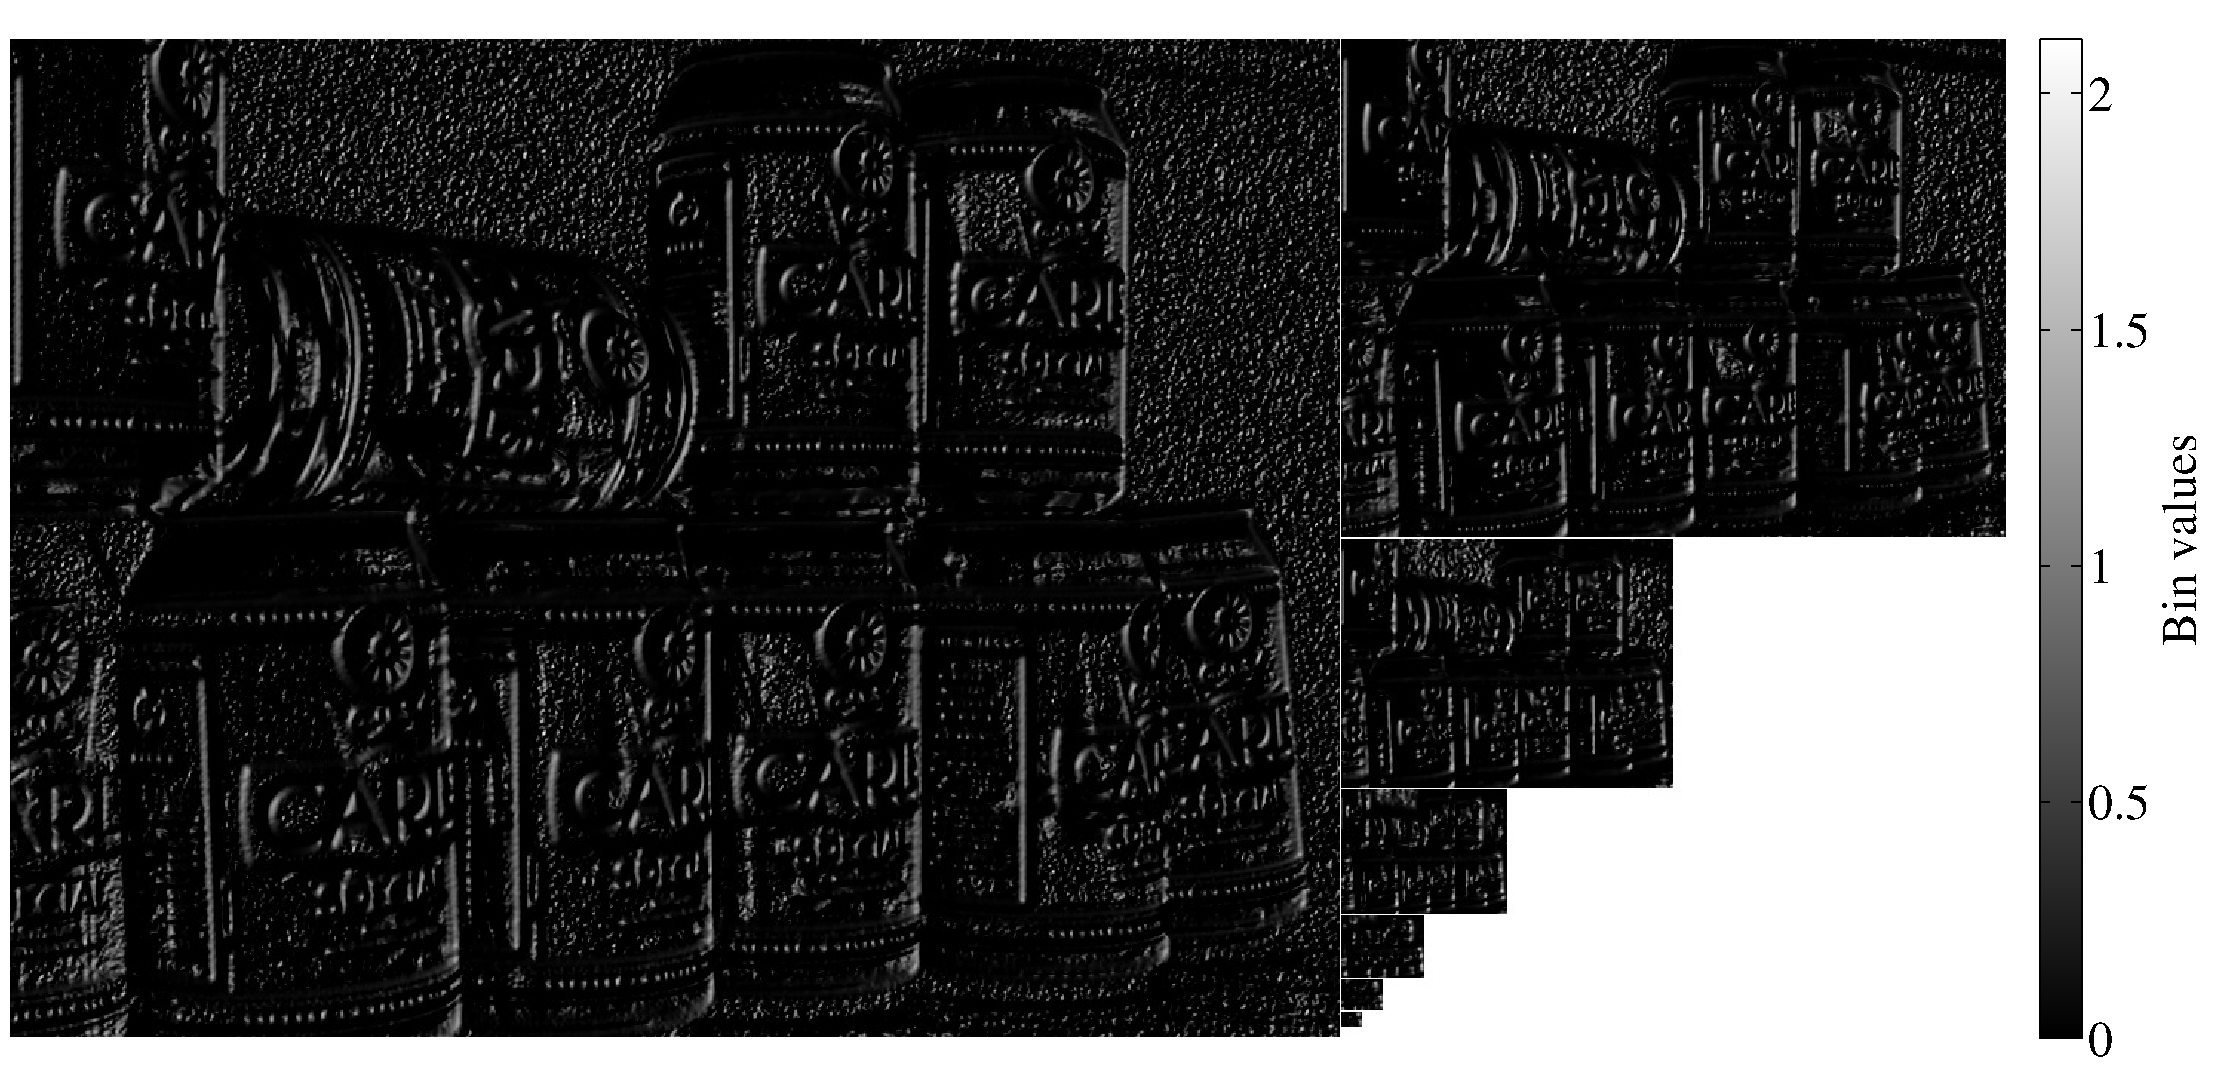
\includegraphics[width=\textwidth]{img/cellHistScaleSpacesBin01.pdf}
    	\caption{Bin $1$ of $8$}
    	\label{fig:cellHistScaleSpacesBin01}
	\end{subfigure}
	\begin{subfigure}[t]{\textwidth}
		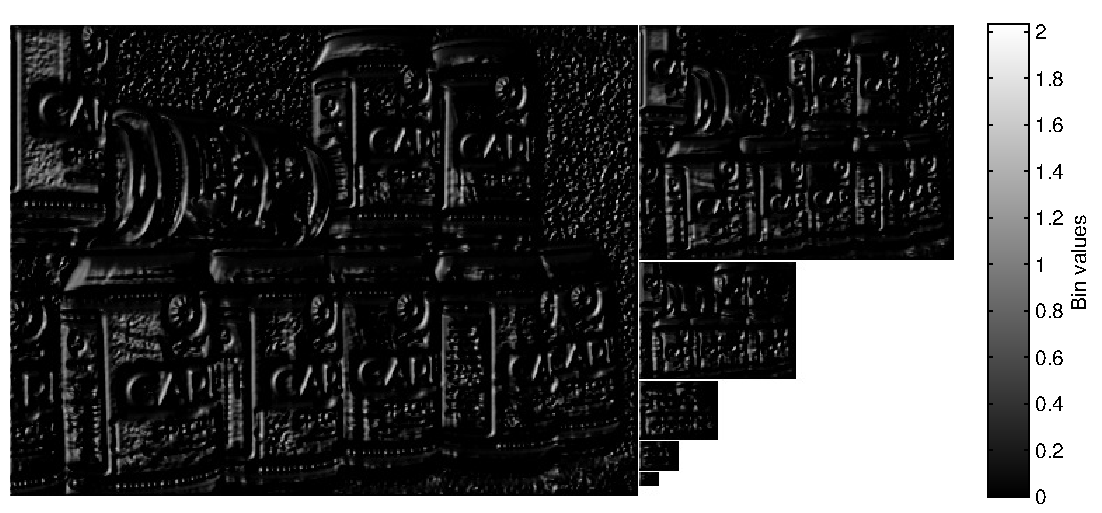
\includegraphics[width=\textwidth]{img/cellHistScaleSpacesBin05.pdf}
    	\caption{Bin $5$ of $8$}
    	\label{fig:cellHistScaleSpacesBin05}
	\end{subfigure}
	\caption{Bin value images for two of the histogram bins. Images \subref{fig:cellHistScaleSpacesBin01} and \subref{fig:cellHistScaleSpacesBin05} correspond to the opposite bin centers $\Theta = -157.5^\circ$ and $\Theta = 22.5^\circ$, and we see that opposite sides of the beer cans are given the greatest bin values for each image.}
	\label{fig:cellHistScaleSpacesBins}
\end{figure}

\begin{figure}[tb]
    \centering
    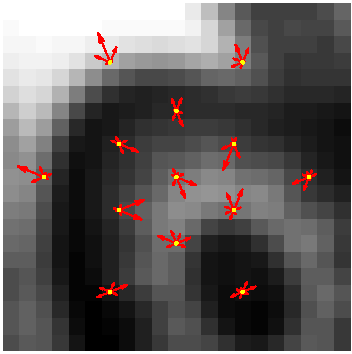
\includegraphics[width=0.65\textwidth]{img/cellHistFigure.pdf}
    \caption{The cell histograms for a single feature that make up our descriptor. For each cell center (yellow), the weighted histogram values (red) are drawn in the direction of the corresponding bin center orientations. We see that the cell histograms generally point towards larger intensities.}
    \label{fig:cellHistFigureGoM}
\end{figure}

\begin{figure}[p]
   	\centering
	\begin{subfigure}[t]{0.65\textwidth}
	    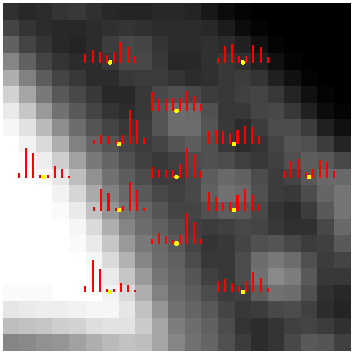
\includegraphics[width=\textwidth]{img/cellHistFigureSi.pdf}
    \end{subfigure}
    \begin{subfigure}[t]{0.9\textwidth}
    	\centering
    	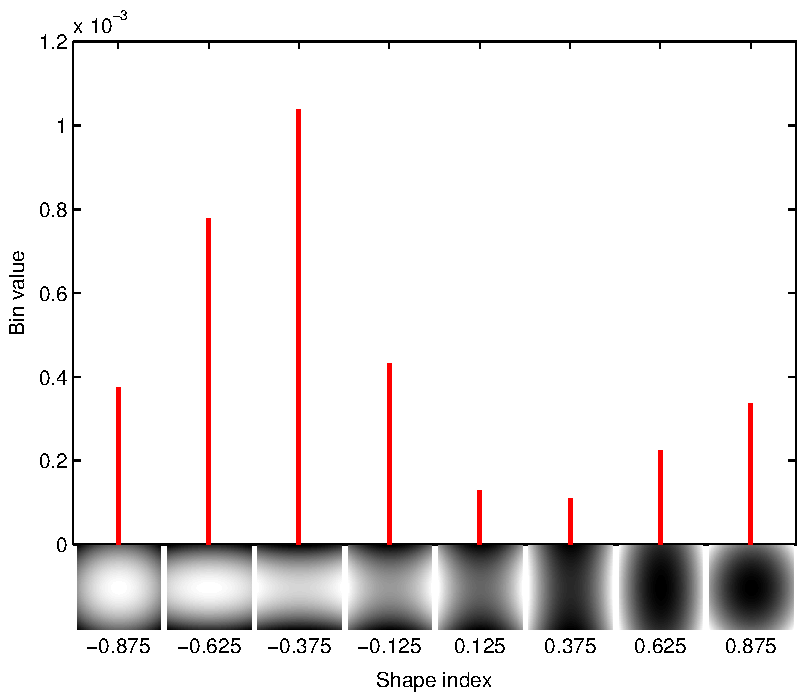
\includegraphics[width=\textwidth]{img/cellHistFigureSiExample.pdf}
%   	\end{subfigure}
%   	\begin{subfigure}[t]{0.1\textwidth}
   	\end{subfigure}
   	\caption{The shape index cell histograms for a single feature.}
    \label{fig:cellHistFigureSiC}
\end{figure}
%
%\section{Notes}
%
% Example scene 47!
%
%\begin{enumerate}
%\item Calculate absolute parameters
%\item Approximate scales needed
%\item Example of detector output
%\item Create scale spaces (approx scales included)
%	Implementation: Chain/direct, Gaussian/finite difference
%	Figures: Examples of scale space images and their corresponding features
%\item Calculate content (gradient orientation, shape index) and magnitudes (gradient magnitude $M$, curvedness $C$)
%	Figures: Go, si examples
%\item Optional: Pixel normalization of magnitudes
%	Figures: Already produced
%\item Create cell indices (in scalespaces), remove interest points too close to the edge, compute cell and center weights
%	Figures: Removed points, maybe some way of displaying weights
%\item Extract magnitudes and values for all image positions inside any cell window
%	Figures: intersection and union of cells
%\item Compute bin weights and renormalize based on bin area and periodicity
%	Figures: 
%\item Compute histogram for each cell by multiplying the bin weights, cell weights, magnitudes, and center weights.
%\item Optional: Normalize each cell histogram
%\item Concatenate cell histograms into feature vectors and normalize
%\end{enumerate}
%
\subbibliography

\end{document}
